\section{Servomotor}

\hookframe{El Servomotor}

\begin{frame}{¿Qué es un Servomotor?}
  \begin{columns}
    \begin{column}{0.6\textwidth}
      Es un dispositivo actuador capaz de:
      \begin{itemize}
        \item Ubicarse en cualquier posición dentro de su rango.\n        \item Mantenerse estable en dicha posición.\n        \item Reaccionar a una señal de control externa.\n      \end{itemize}
      \vspace{0.5cm}
      \textbf{Uso común:} Robótica, aeromodelismo y sistemas de control de precisión.
    \end{column}
    \begin{column}{0.4\textwidth}
      \centering
      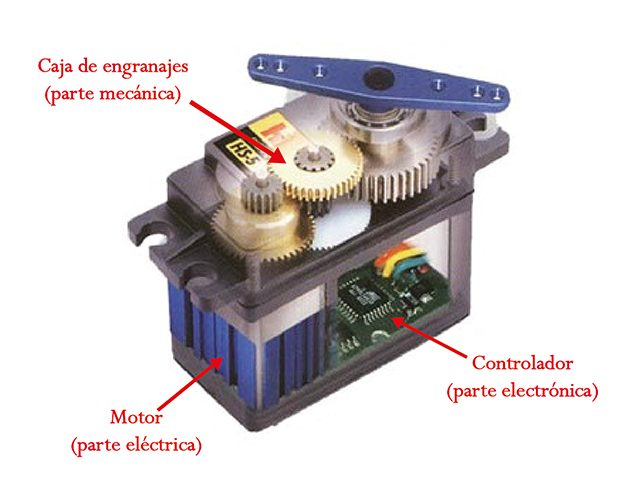
\includegraphics[width=\textwidth]{../images/servo/servomotor}
      \caption{Servo de modelismo}
    \end{column}
  \end{columns}
\end{frame}

\begin{frame}{Anatomía Interna}
  Un servomotor no es solo un motor, es un \textbf{sistema cerrado} compuesto por:
  \vspace{0.3cm}
  \begin{enumerate}
    \item \textbf{Motor DC:} El músculo (alta velocidad, bajo par).\n    \item \textbf{Caja Reductora:} El multiplicador de fuerza (baja velocidad, alto par).\n    \item \textbf{Circuito de Control:} El cerebro (procesa la señal y el error).\n    \item \textbf{Potenciómetro:} El sensor de posición (realimentación).\n  \end{enumerate}
  \vspace{0.3cm}
  \centering
  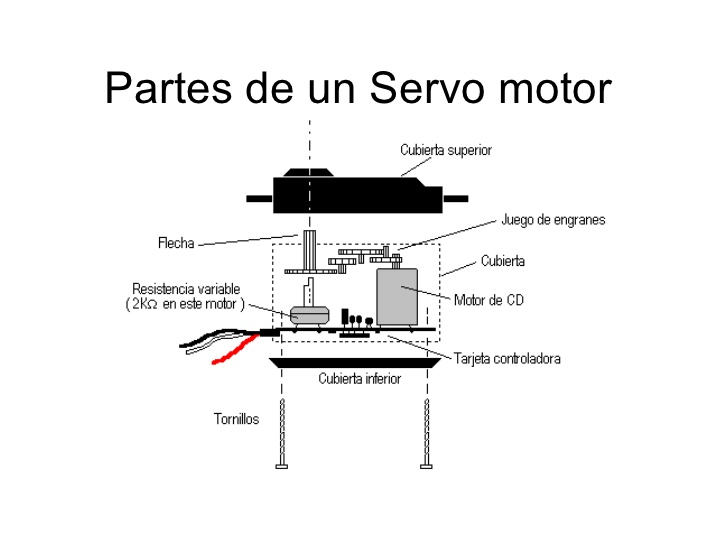
\includegraphics[width=0.6\textwidth]{../images/servo/partservo}
\end{frame}

\begin{frame}{El Control: Señal PWM}
  \begin{block}{Setpoint (Punto de Referencia)}
    La posición deseada se indica mediante una señal cuadrada de ancho de pulso variable (PWM).
  \end{block}
  \vspace{0.3cm}
  \begin{itemize}
    \item \textbf{Pulso más ancho} $\rightarrow$ Ángulo mayor.\n    \item \textbf{Pulso más estrecho} $\rightarrow$ Ángulo menor.\n  \end{itemize}
  \centering
  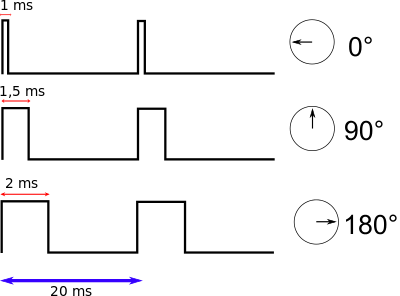
\includegraphics[width=0.7\textwidth]{../images/servo/pwm}
\end{frame}

\begin{frame}{El Lazo de Realimentación}
  \centering
  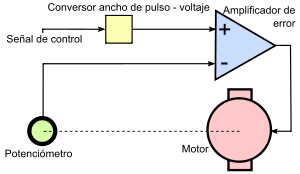
\includegraphics[width=0.8\textwidth]{../images/servo/servo}
  \vspace{0.3cm}
  \begin{itemize}
    \item El \textbf{potenciómetro} mide la posición real.\n    \item El \textbf{amplificador de error} resta: $\text{Error} = \text{Referencia} - \text{Posición Real}$.\n    \item Si el error $\neq 0$, el motor gira hasta que la diferencia desaparezca.\n  \end{itemize}
\end{frame}

\begin{frame}{La Matemática del Posicionamiento}
  Para un servo estándar ($0^o$ a $180^o$) con pulsos de $1\text{ms}$ a $2\text{ms}$:
  \vspace{0.5cm}
  \begin{equation}
    t = 1 + \frac{\phi}{180}
  \end{equation}
  \vspace{0.5cm}
  \begin{itemize}
    \item $t$: Duración del pulso en milisegundos (ms).\n    \item $\phi$: Ángulo deseado en grados ($^o$).\n  \end{itemize}
  \vspace{0.3cm}
  \begin{exampleblock}{Ejemplo}
    Para posicionar el servo a $90^o$: $t = 1 + \frac{90}{180} = 1.5\text{ms}$.
  \end{exampleblock}
\end{frame}

\begin{frame}{Tip Práctico: El Bloqueo del Servo}
  \begin{alertblock}{Importante}
    Para que el servo resista fuerzas externas y mantenga su posición, debe recibir la señal de control \textbf{continuamente}.
  \end{alertblock}
  \vspace{0.5cm}
  \begin{itemize}
    \item \textbf{Con señal:} El sistema corrige activamente cualquier desviación.\n    \item \textbf{Sin señal:} El motor queda liberado y puede ser movido manualmente.\n  \end{itemize}
\end{frame}

\begin{frame}{Check de Comprensión}
  \begin{enumerate}
    \item ¿Por qué es necesaria la caja reductora si ya tenemos un motor DC?\n    \item ¿Qué sucede físicamente en el circuito si el error de posición es cero?\n    \item Si quiero mover el servo a $45^o$, ¿cuál debe ser la duración del pulso?\n  \end{enumerate}
\end{frame}